\section{Discussion: The Usability Trap \& Metric Refinement}
\label{sec:discussion}

The interplay between identity disruption, network containment, and client breakage exposes structural deficiencies in naive privacy-usability metrics. 
Here, we deconstruct the failure of our initial metric formulation, present the axiomatic derivation of the Refined Effectiveness-to-Risk metric ($\etr$), and map the empirical Pareto frontier governing browser privacy.

\subsection{Deconstructing the Usability Trap}
\label{subsec:usability_trap}

Initial privacy measurement frameworks often model the trade-off between tracking mitigation and usability via intuitive composite quotients. We initially benchmarked browser configurations using the formulation:
\begin{equation}
\etrinit = \frac{(1 - \rid) \times \left( \frac{1}{\ln(D_{\text{ID}} + e)} \right)}{1 + \ucost}
\label{eq:etr_initial}
\end{equation}
Evaluating our empirical corpus under Equation~\ref{eq:etr_initial} produced an anomalous, inverted ranking:
\begin{align*}
\etrinit: \; & \text{FF Base (0.046)} > \text{FF Hard (0.042)} > \text{Chrome (0.040)} \\
& > \text{Brave Base (0.035)} > \text{Brave Hard (0.035)}
\end{align*}
This formulation ranked completely unhardened Chrome ($0.0395$) \textit{higher} than Brave Hardened ($0.0347$), despite the latter destroying $60\%$ of auction clearing revenue and capping the upper quartile at $Q_3 = 0.00\%$. 
Forensic analysis revealed three mathematical pathologies:

\paragraph{1. Binary Disruption Insensitivity}
The binary re-identification rate $\rid$ registers an active domain as ``tracked'' if $\Delta\cpm \ge -10\%$. This threshold creates a step-function discontinuity that ignores deep economic disruption: a minor drop of $-11\%$ is treated identically to complete market annihilation ($-100.0\%$). 
Consequently, Brave Hardened's median collapse ($-59.98\%$) and $25\%$ total wipeout rate were completely discarded by the numerator.

\paragraph{2. Linear Denominator Penalty}
The linear denominator ($1 + \ucost = 1.44$) penalized Brave Hardened by $44\%$, disproportionately degrading its score and drowning out its substantial privacy gains.

\paragraph{3. The Retry-Storm Inversion}
Equation~\ref{eq:etr_initial} uses raw identity diffusion events ($D_{\text{ID}}$) in the logarithmic denominator. As revealed in Section~\ref{subsec:silo_network}, blocking tracker endpoints triggers client-side retry storms: client scripts repeatedly re-trigger cookie synchronization~\cite{papadopoulos2019cookie} and UID decoration loops~\cite{randall2022measuring} within recursive event handlers~\cite{iqbal2020adgraph}. 
This paradoxically inflated Hardened Firefox's diffusion volume to 28,976 total events (6,006 cookie syncs and 22,970 smuggled UIDs), penalizing the browser for effectively blocking third-party endpoints.

\subsection{Axiomatic Formulation of $\etr$}
\label{subsec:etr_star}

To resolve these distortions, we formulate the \textbf{Refined Effectiveness-to-Risk Metric} ($\etr$):
\begin{equation}
\etr = \frac{\Phi_{\text{econ}} \times \Psi_{\text{containment}}}{\Omega_{\text{usability}}}
\label{eq:etr_refined}
\end{equation}
where each component satisfies strict axiomatic requirements:

\paragraph{Continuous Economic Disruption ($\Phi_{\text{econ}}$)}
We replace the binary factor $(1 - \rid)$ with a composite economic index that integrates binary resistance, high-tier disruption, and median price decay:
\begin{equation}
\Phi_{\text{econ}} = \frac{(1 - \rid) + \htr + \max(0, -\widetilde{\Delta\cpm})}{3}
\end{equation}
where $\widetilde{\Delta\cpm}$ is the median relative bid shift. $\Phi_{\text{econ}} \in [0, 1]$ scales monotonically with both the breadth ($\htr$) and depth ($-\widetilde{\Delta\cpm}$) of tracking disruption.

\paragraph{Entity Density Containment ($\Psi_{\text{containment}}$)}
To eliminate retry-storm artifacts, we replace raw request counts with the density of unique tracking entities contacted per publisher:
\begin{equation}
\Psi_{\text{containment}} = \frac{1}{\ln\left(\frac{D_{\text{entity}}}{N_{\text{sites}}} + e\right)}
\end{equation}
where $D_{\text{entity}}$ is the count of deduplicated third-party hosts and $N_{\text{sites}} = 150$. By evaluating host density ($d = D_{\text{entity}} / 150$), $\Psi$ rewards browsers that restrict communication across distinct corporate tracking entities~\cite{bashir2016tracing, cook2020inferring}, remaining invariant to local script retry loops. As $D_{\text{entity}} \to 0$, $\Psi \to 1.0$.

\paragraph{Sub-Linear Usability Dampening ($\Omega_{\text{usability}}$)}
To prevent script exceptions from disproportionately penalizing privacy gains, we dampen the usability penalty logarithmically:
\begin{equation}
\Omega_{\text{usability}} = 1 + \ln(1 + \ucost)
\end{equation}
This dampens the impact of script errors, ensuring that browsers achieving deep privacy protection are not penalized below unhardened baselines.

\begin{table}[t]
\centering
\small
\caption{Decomposition of Refined Metric Components ($\etr$). Deduplicated tracking host density restores monotonically sound defense rankings.}
\label{tab:etr_breakdown}
\resizebox{\columnwidth}{!}{%
\begin{tabular}{lcccccc}
\toprule
\textbf{Configuration} & $\Phi_{\text{econ}}$ & $\frac{D_{\text{entity}}}{N}$ & $\Psi_{\text{cont}}$ & $\Omega_{\text{use}}$ & $\etr$ & \textbf{Rank} \\
\midrule
\texttt{chrome\_baseline}  & 0.226 & 5.813 & 0.467 & 1.000 & \textbf{0.105} & Control \\
\texttt{firefox\_baseline} & 0.289 & 5.613 & 0.471 & 1.000 & \textbf{0.136} & Dominated \\
\texttt{brave\_baseline}   & 0.322 & 5.760 & 0.468 & 1.270 & \textbf{0.131} & Dominated \\
\texttt{firefox\_hardened} & 0.368 & \textbf{5.400} & \textbf{0.476} & 1.000 & \textbf{0.175} & Pareto Apex \\
\texttt{brave\_hardened}   & \textbf{0.526} & 5.920 & 0.465 & 1.365 & \textbf{0.179} & Pareto Apex \\
\bottomrule
\end{tabular}%
}
\end{table}

\paragraph{Benchmark Restoration}
As demonstrated in Table~\ref{tab:etr_breakdown}, $\etr$ restores a consistent ranking:
\begin{align*}
\etr: \;\; & \text{Brave Hard (0.179)} > \text{FF Hard (0.175)} > \text{FF Base (0.136)} \\
& > \text{Brave Base (0.131)} > \text{Chrome Base (0.105)}
\end{align*}
Unhardened Chrome correctly anchors the bottom of the benchmark, while Hardened Brave and Hardened Firefox share the upper bound through complementary trade-offs.

\subsection{The Empirical Pareto Frontier}
\label{subsec:pareto_frontier}

Our empirical findings demonstrate that client-side web privacy adheres to a multi-objective Pareto optimization problem: maximizing economic tracking disruption ($\Phi_{\text{econ}}$) while minimizing usability breakage ($\ucost$).

\begin{figure}[t]
\centering
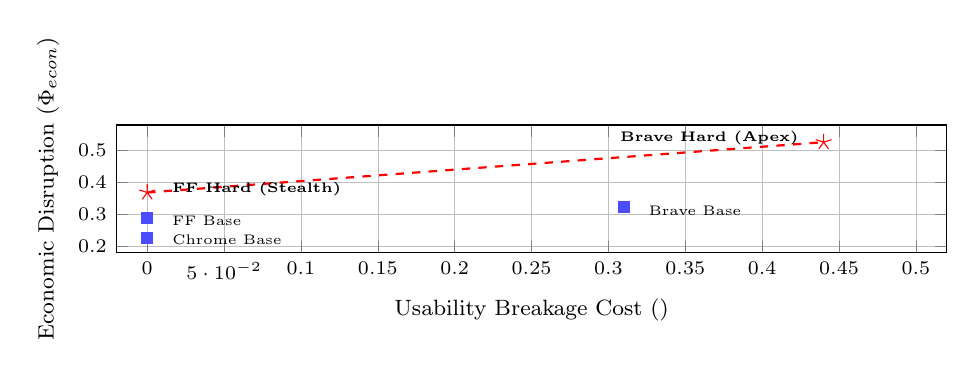
\begin{tikzpicture}
\begin{axis}[
    width=\columnwidth,
    height=3.2cm,
    xlabel={Usability Breakage Cost ($\ucost$)},
    ylabel={Economic Disruption ($\Phi_{\text{econ}}$)},
    xlabel style={font=\footnotesize},
    ylabel style={font=\footnotesize},
    ticklabel style={font=\scriptsize},
    xmin=-0.02, xmax=0.52,
    ymin=0.18, ymax=0.58,
    grid=both,
    grid style={line width=.1pt, draw=gray!20},
    major grid style={line width=.2pt,draw=gray!50}
]

% Pareto Frontier Line
\addplot[thick, dashed, red] coordinates {
    (0.00, 0.368) % FF Hard
    (0.44, 0.526) % Brave Hard
};

% Non-dominated Pareto Optimal Points
\addplot[only marks, mark=star, mark size=3.0pt, red] coordinates {
    (0.00, 0.368) % FF Hardened
    (0.44, 0.526) % Brave Hardened
};

% Dominated Points
\addplot[only marks, mark=square*, mark size=2.0pt, blue!70] coordinates {
    (0.00, 0.226) % Chrome
    (0.00, 0.289) % FF Base
    (0.31, 0.322) % Brave Base
};

% Labels with manual offset to avoid margin collision
\node[anchor=west, font=\tiny] at (axis cs:0.01,0.38) {\textbf{FF Hard (Stealth)}};
\node[anchor=east, font=\tiny] at (axis cs:0.43,0.54) {\textbf{Brave Hard (Apex)}};
\node[anchor=west, font=\tiny] at (axis cs:0.01,0.22) {Chrome Base};
\node[anchor=west, font=\tiny] at (axis cs:0.01,0.28) {FF Base};
\node[anchor=west, font=\tiny] at (axis cs:0.32,0.31) {Brave Base};

\end{axis}
\end{tikzpicture}
\caption{The Empirical Privacy-Usability Pareto Frontier. The red dashed line connects the non-dominated Pareto boundaries: Stealth Optimum (FF Hardened) and Apex Disruption (Brave Hardened).}
\label{fig:pareto}
\end{figure}

As mapped in Figure~\ref{fig:pareto}, defense strategies define an empirical frontier:
\begin{enumerate}
    \item \textbf{The Stealth / Zero-Breakage Optimum (\texttt{firefox\_hardened}):} Combining Tor-derived API normalization (RFP)~\cite{tor_design, mozilla_rfp_docs} with Total Cookie Protection and query stripping~\cite{randall2022measuring} achieves $\Phi_{\text{econ}} = 0.368$ (a $-26.86\%$ median bid collapse) with \textbf{zero usability breakage ($\ucost = 0.00$)}. 
    Because RFP normalizes API return values to uniform mock pools rather than severing network calls, downstream publisher code continues executing cleanly.
    \item \textbf{The Maximum Privacy Optimum (\texttt{brave\_hardened}):} Combining API farbling~\cite{brave_fingerprinting_protections_2025} with aggressive network-level blocking maximizes tracking severance ($\Phi_{\text{econ}} = 0.526$, $-59.98\%$ median collapse, $\rid = 0.500$), but incurs $\ucost = 0.44$ due to severed script dependency chains~\cite{iqbal2020adgraph}. 
    \item \textbf{Dominated Configurations:} \nolinkurl{chrome_baseline}, \nolinkurl{firefox_baseline}, and \nolinkurl{brave_baseline} are strictly Pareto-dominated, yielding weaker privacy protections without offering offsetting usability advantages.
\end{enumerate}

\subsection{Methodological Post-Mortem}
\label{subsec:post_mortem}

During platform validation, we identified a critical experimental failure mode: naive filesystem profile cloning leaked persistent identifiers across phases. 
Chromium caches session descriptors and HSTS tokens within binary LevelDB transaction logs and service worker quotas. In early test runs, unpurged LevelDB files preserved cross-phase identity state, producing artificial $0.0\%$ bid shifts.

This failure confirms empirical findings by Acar et al.~\cite{acar2014web} and Lerner et al.~\cite{lerner2016internet}, who demonstrated that commercial tracking networks exploit persistent HTML5 Web Storage~\cite{whatwg_webstorage} and HSTS supercookies to respawn deleted identifiers. 
Standard browser ``Clear Browsing Data'' routines are insufficient for rigorous web measurement; reliable causal interventions require deterministic profile sanitization that wipes underlying LevelDB stores while preserving anti-fingerprinting defenses.